%! Author = vsharma
%! Date = 25.09.2022
% !TeX spellcheck = en_EN

\chapter{Related Work}

\section{Cloud Background}

\subsection{Cloud Computing}
Cloud computing in simple terms is defined as the delivery of computing services and resources.
These include
storage, databases, servers, software, and networking over the internet.
Cloud computing is a combination of two
words “cloud” which means “internet” and computing involves the systems and infrastructures that enable a computer to run and build, deploy, or interact with information.
Cloud computing is a very common phrase that people hear nowadays but might not actually understand.
It is because cloud computing encompasses several different services and systems thus making it ambiguous or confusing.
Delivery of computing services such as servers, databases, storage, etc. over the internet is defined as cloud computing \cite{11}.

Cloud computing enables the use of off-site systems which helps the computers to store, manage, process, and
communicate information.
These services are not posted on-premises by the
organization rather they are accessible over the internet.
These systems can store anything from software programs to email servers, data storage, etc \cite{11}
\cite{12}.

\subsection{Types of cloud computing:}

\par There are different cloud providers that offer cloud services namely Amazon Web Services (AWS), the cloud computing service of Amazon.com, Microsoft Corporation’s cloud segment contains Azure, Google Cloud Platform (GCP), part of Alphabet Inc, etc.
Each of the cloud platforms is unique in its own way and offers a plethora of options for organizations to select from based on their specific requirements.
When considering the services offered by these clouds,
Google Cloud offers up to 60+ services, whereas Azure
offers around 100+ services.
AWS, on the other hand, offers around 200+ services.
In terms of the availability zones, AWS has 66
availability zones, Azure has 54 regions worldwide and is
available in 140 countries all around the world, and
\gls{gcp} has been made available in
20 regions around the world \cite{13}.
While deciding on a cloud service provider there are
several factors that needs to be considered.
In order to determine the most suitable type of cloud computing on which the cloud services can be implemented, it is better to first identify the type of cloud computing architecture or cloud deployment.
There are three different cloud offerings to deploy cloud services: a private cloud, a public cloud, or a hybrid cloud \cite{14}.
\hfill \break
\textbf{Private cloud:}
Private cloud refers to computing resources that are used by a particular organization or a single business.
In this,
the computing resources are owned, operated, and governed by the same organization.
The cloud
computing resources are physically located at the
organization’s on-site datacenter in the private cloud, the
services
and
the
infrastructure are maintained by a private network \cite{14}.
\hfill \break
\textbf{Public cloud:}
This type of cloud usually offers B2C (Business to Consumer) type of interactions. Public clouds are operated and
owned by a third-party cloud service provider which delivers these resources over the internet. AWS is an example of
a public cloud where the cloud service provider owns and manages all the software, hardware, and other supporting
services \cite{14}.
\hfill \break
\textbf{Hybrid cloud:}
A hybrid cloud refers to the mixed storage, services, and computing environment comprises of a public cloud such as
AWS and an on-premises infrastructure, a private cloud. The hybrid cloud approach is the most widely used infrastructure configuration these days as it enables the organization
to continue using their on-premises servers while taking the advantage of available public cloud options like AWS,
and Azure. This enables the organization to comply with the data residency policies while leveraging the benefits and
security of the public cloud \cite{14}.


\subsection{Types of cloud services:}
\textbf{Infrastructure as a service (IaaS)}
\par This type of cloud computing service offers
essential storage, memory, compute, and related networking, such as
operating systems and databases, as a cloud service to replace the on-premises infrastructure.
In a typical IaaS
architecture, the most essential components are hosted by the cloud providers such as Networking hardware, Servers, Storage, Physical hardware, etc. This feature enables IaaS to provide the same capabilities and technologies as offered by the traditional on-premises data centers \cite{9}. The customer needs to only perform a few steps:
\begin{itemize}
    \item Customers can access the services over the internet by logging in to the IaaS platform created by the cloud
    service provider \cite{15}.
\end{itemize}
\begin{itemize}
    \item The customer is then required to create a Virtual
    Machine (VMs) on the cloud platform according to their
    requirements and then install the operating system
    (OS) on the VMs. Once the OS is deployed on the VM,
    the customer must deploy middleware, create
    storage buckets to hold the workloads and backups, and
    install the enterprise workload into that VM \cite{15}.
\end{itemize}
\begin{itemize}
    \item Finally, these VMs can be deployed along with databases, apps, desired tools, and the company’s workload \cite{15}.
\end{itemize}
IaaS benefits businesses by reducing operating costs, and by spending less on software upgrades and maintenance
\cite{15}.

\begin{figure}
    \centering
    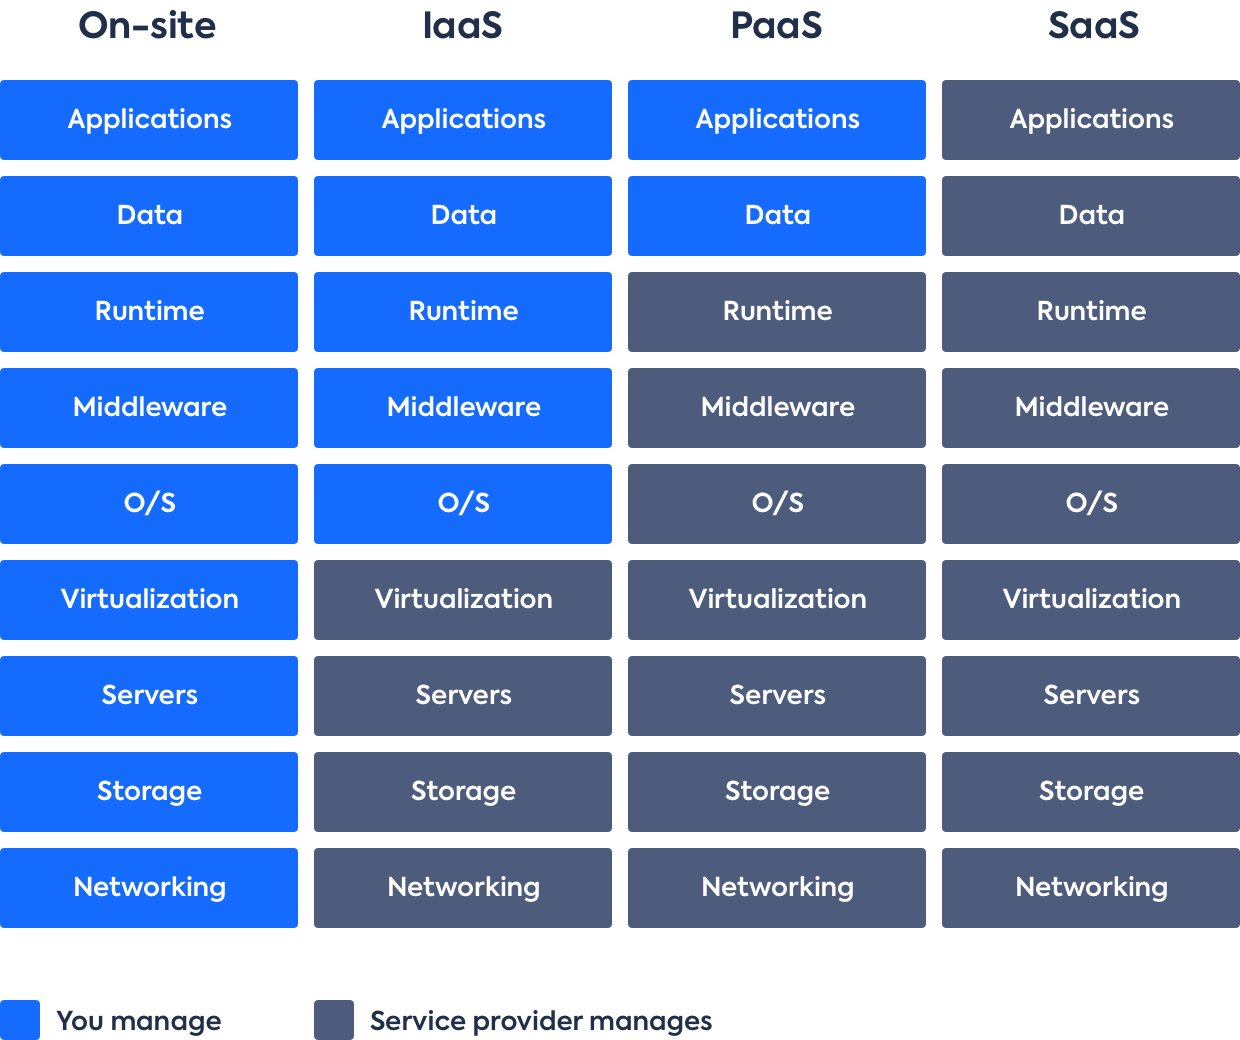
\includegraphics[width=\textwidth]{iaaspaassaas.jpg}
    \caption{Cloud computing models}{\cite{16}}
    \label{fig:iaaspaassaas}
\end{figure}

\clearpage
\textbf{Platform as a service (PaaS)}
\par \gls{paas} is a model that provides cloud-based
services
enabling the developers and businesses to build software
and applications at a faster speed that could not be
achieved in on-premises solutions.
It is an on-demand service providing companies with a
complete set of software, hardware, and infrastructure for
developing, running, testing, and managing software
applications and eliminates the complexity and expense of
buying, evaluating, configuring, and managing all the
required software and hardware needed for applications.
It provides the organization with a cost-effective,
complete, and flexible platform.
It allows programmers to develop web and mobile
applications without worrying about managing or setting up the underlying infrastructure for storage, servers, databases, and networks that are needed for deployment \cite{15}.


\par With PaaS, the organization avoids the complexity and expense of buying the software licenses, the underlying infrastructure, container orchestrators, development tools, and middleware or other resources.
The organization only manages the application developed
by them and cloud service providers such as Amazon AWS
manage everything else \cite{15}.\\

\hfill \break

\textbf{Software as a service (SaaS)}
\par \gls{saas} is a method of delivering software and
application
to the end user over the internet.
These applications can be accessed via the
mobile application, internet browser, or desktop app.
Common examples of SaaS are calendaring, email, and office tools (such as Microsoft Office 365).
It is a distribution model in which the applications are hosted by cloud service providers or vendors to users across the globe.
The another name given to these applications are
on-demand
software, Web-based software, or hosted software and run
on the provider's servers.
The provider takes all the responsibilities of managing the application that includes performance, availability and security.
SaaS offers a subscription-based model
which
means users pay recurring monthly or annual fees for
using the product, the user don’t need to worry
about the huge
upfront cost.
In SaaS, all the
application software, middleware, application data, and infrastructure are in the cloud service provider’s data center.
The software resources and hardware resources are managed
by the
cloud
service provider.
The availability and security of data and applications in the cloud are also ensured by cloud service providers.
It enables bringing up the organization’s application and
running quickly and at a minimal upfront cost \cite{15}.

\par Figure \ref{fig:iaaspaassaas} describes the responsibilities of each deployment model compared to the on-premises setup.

\section{Amazon Web Services}
\par This section introduces the relevant AWS services and associated terminology used in this thesis. It is written to provide the reader with ample background knowledge required to understand this research work. It therefore by no means introduces the entire AWS platform.

\subsection{General AWS background}

\par Amazon web services is an evolving cloud computing subsidiary of Amazon.
Amazon Web
Services portfolio comprises more than 200+ services including database, compute, application
development, security, infrastructure management, analytics, migration, etc.
that help the
organization to scale and grow.
For example, AWS provides a wide range of databases that are
designed specifically for specific applications.
AWS combines the offerings of the three cloud services 
namely PaaS, IaaS, and SaaS \cite{17}.

\par AWS was launched in 2006 and was one of the first
cloud service providers to introduce a pay-as-you-go cloud computing model. It offers various tools and solutions for developers \cite{18}.

\par AWS cloud infrastructure is a highly secure,
reliable, and extensive cloud platform \cite{19}. Whether
it is required to deploy the application workloads
globally with just one click, or to develop and deploy specific applications closer to the end user with latency in the single-digit millisecond range, AWS offers the right cloud infrastructure anywhere, anytime \cite{20}.

\begin{itemize}
    \item AWS Regions
    \item Availability zones
    \item Edge locations
\end{itemize}

\begin{figure}
    \centering
    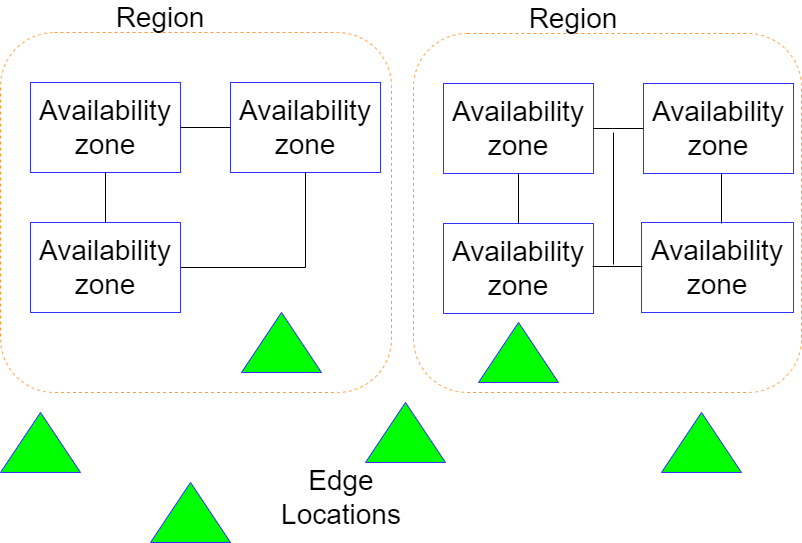
\includegraphics[width=\textwidth]{geographicalcomponents.png}
    \caption{AWS Geographical Components}{\cite{16}}
    \label{fig:identities}
\end{figure}

\par When designing and architecting the cloud infrastructure it is very important to know where the instances, services are data are located.
This is a fundamental criterion to implement a highly
available and scalable network that offers low latency
\cite{20}.


\textbf{Region}
\par Regions are geographical locations to operate and run cloud services.
These regions are spread globally and reduce the latency incurred by the customer when accessing the resource.
Each AWS region contains availability zones.
For each AWS region, there are a minimum of 2 Availability
Zones and a
maximum of 6 Availability Zones, however typically 3 or more are usually found.
The regions are connected to one another via a high-speed
fiber network and are isolated from each other \cite{21}


\textbf{Availability zones}
\par Every AWS region is made up of \textit{AWS Availability Zone (AZ)} which are the logical building block. Each AZ is isolated from other AZ for the failures.
The AWS regions operate independently and are isolated from other regions, but the availability zone within a region provides low-latency network connectivity to other Availability Zones within the same AWS Region.
There is no explicit cost incurred for the network connectivity between two Availability Zones within the same AWS Region.
Depending on the service used, in case of a failure, if an Availability Zone goes down, it is possible to ensure high availability by shifting the workload to another Availability Zone within the same region, this capability is known as \textit{Multi-AZ} redundancy.
The figure \ref{fig:identities} shows 2 different AWS
regions which are isolated from each other and each region consists of AWS Availability Zones \cite{22}.

\textbf{Edge Location}
\par In order to reduce the latency for the traffic, edge locations are deployed at multiple locations across the
world. Edge locations limit to building a new data center
if the customers are in different cities, a different
state, a different
country or a different
part of the world. Edge locations can be understood as servers that are placed geographically close to the clients.
If we consider an example, an organization has many clients in Tokyo accessing the information which is deployed in a
region in Mumbai. In such cases, instead of clients sending requests constantly to Mumbai region for accessing the
information, we can cache a copy of the relevant information in Tokyo. Amazon CloudFront allows delivering video,
information, APIs to clients, or applications across the world. AWS CloudFront uses edge locations for accelerating
communication with customers \cite{23}.

\subsection{Services}

\textbf{AWS Identity and Access Management (IAM)}

\par Amazon \gls{iam} is a web service that helps to
securely
control access for the users to Amazon Web Services resources and services.
Using IAM enables creating and managing Amazon Web Services groups and users and uses permissions to allow and deny their permissions to AWS resources.
IAM enables organizations to create and control services
for user authentication or limit access to a certain set of people who use their AWS resources \cite{24}.


\par When an AWS account is created, it begins with one
sign-in identity.
This identity has
complete access to all AWS resources and services in the account and is called the \textit{root user}.
The AWS account root
user is accessed by signing in with the email address and password that you used to create the account.
As
recommended, the usage of root users must be avoided for
everyday tasks \cite{25}.


\begin{figure}
    \centering
    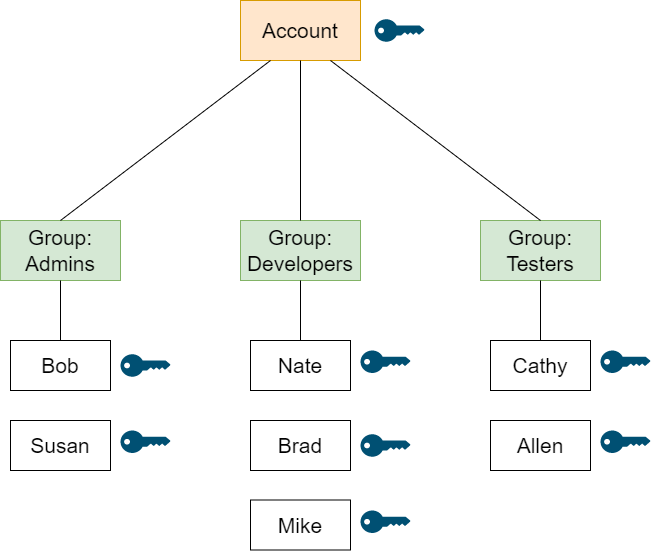
\includegraphics[width=\textwidth]{groupusers.png}
    \caption{IAM users and groups}{\cite{26}}
    \label{fig:groupusers}
\end{figure}

\textbf{IAM Users}

\par An IAM user represents an entity within the AWS account.
This entity corresponds to an application or a person and has specific permissions.
Users have their own set of authentication parameters such as access key, secret key, or password that is required to access the AWS account through CLI or AWS console.
An IAM user does not always represent an actual individual.
Each IAM user is associated with only one AWS account
\cite{27}.
\hfill \break

\textbf{IAM Group}
\par An IAM group is an identity that specifies a 
collection of IAM users as shown in figure \ref{fig:groupusers}.
The user
groups help in specifying the permissions for multiple users, thus making it easier to manage the permissions for the users.
For example, there could be a user group in an organization called Admins that provides all users administrator permissions who belong to that user group.
If a new user joins the organization and should have administrator privileges, just by adding the new user to the admin user group, the user can be assigned the required permissions.
Similarly, if a user changes a job role within the organization, instead of editing that user’s permissions, it is possible to simply remove them from the old user groups and add them to the new user groups \cite{27}.
\hfill \break


\textbf{Roles}
\par An IAM role is not associated with a specific person,
but it is similar to an IAM user.
A role can be assumed
temporarily by switching the roles in the management
console of AWS. It is also possible to assume a role
through the AWS API operation or by calling the AWS
\gls{cli}
or by using a custom URL.
There are no standard long-term credentials such as passwords or access keys associated with a role.
A role provides a temporary security credentials for the role session when it is assumed.
It is possible to use roles to delegate access to users, services, or applications that don't have access to your AWS resources. For example, it is required to grant users within an AWS account access to resources the users usually don’t have or grant users in one AWS account access to resources in another account \cite{27}.

\hfill \break
\textbf{Policy}

\par An IAM policy is an IAM entity that sets permission and controls access to AWS resources.
The IAM policies are attached to AWS resources or IAM identities (users, groups, or roles) and define their permission.
These policies are evaluated when a principal such as a role or a user makes a request. Most policies in AWS are stored as JSON documents. IAM policies define permissions which specify who has access to the resources and what operation they can perform. For example, if there exists a policy that allows the GetUser action, then if this policy is assigned to the user, the user would be able to fetch the information either by using the AWS API or the AWS CLI or the AWS Management Console \cite{14}.

\par AWS provides six types of policies:

\begin{itemize}
    \item \textbf{Identity-based policies:} Identity-based policies are JSON documents that control what actions an
    identity
    (users, groups, and roles) can perform, under what conditions, and on which resources \cite{27}. The Identity-based policies can be further categorized as:
    \begin{itemize}
        \item Managed policies: Standalone identity-based policies that are attached to multiple users, groups, and
        roles in an AWS account \cite{27}.
    \end{itemize}
    \begin{itemize}
        \item Inline policies:  Policies that are added directly to a single identity such as user, group, or role.
        Inline policies maintain a strict one-to-one relationship between an identity and a policy and are deleted when the identity is deleted \cite{27}.
    \end{itemize}
\end{itemize}

\begin{itemize}
    \item \textbf{Resource-based policies:} Policy document attached to a resource such as an Amazon S3 bucket is known as Resource-based policies.
    These are inline policies and grant the specified permission to perform specific actions on a resource \cite{27}.
\end{itemize}
\begin{itemize}
    \item \textbf{IAM permissions boundaries:} A permissions' boundary sets the maximum permissions that can be granted to an IAM entity by an identity-based policy.
     When the permissions boundary for an entity is set, the entity can perform only the actions that are allowed by both its permissions boundaries and its identity-based policies.
     Permissions boundary does not limit the
    resource-based policies that specify the user or role as the principal \cite{27}.
\end{itemize}
\begin{itemize}
    \item \textbf{Organizations \gls{scp}:} Amazon
    Organizations
    is a service for grouping and centrally managing the Amazon accounts that the business owns.
    It helps to centrally manage and govern the environment as the organization grows and scales its AWS resources.
    The maximun permission for account members of an
    \gls{ou} is defined using
    Amazon
    Organizations.
    AWS OSCP limits the permissions granted to entities i
    .e. users or roles within the account by the
    identity-based policies or resource-based policies,
    but it does not grant permissions \cite{27}.

\end{itemize}
\begin{itemize}
    \item \textbf{Access control lists (ACLs):} ACL is a service policy that allows to control the access to a resource by the principals in another account.
    ACLs are the only policy types that does not uses the JSON policy structure and are similar to resource-based policies.
    ACLs are used to grant permissions to the specified principal since they are cross-account permissions policies.
    Using ACL it is not possible to control the access within the same account \cite{27}.
\end{itemize}
\begin{itemize}
    \item \textbf{Session policies:} Session policies are
    policies used for programmatically creating a temporary session for a federated user or role by passing them as parameters.The intersection of session policies and identity-based policies for the IAM user or role represents the permissions for a session \cite{27}.
\end{itemize}

Figure \ref{fig:iamidentities} shows the overview of AWS IAM concepts in AWS infrastructure.


\begin{figure}
    \centering
    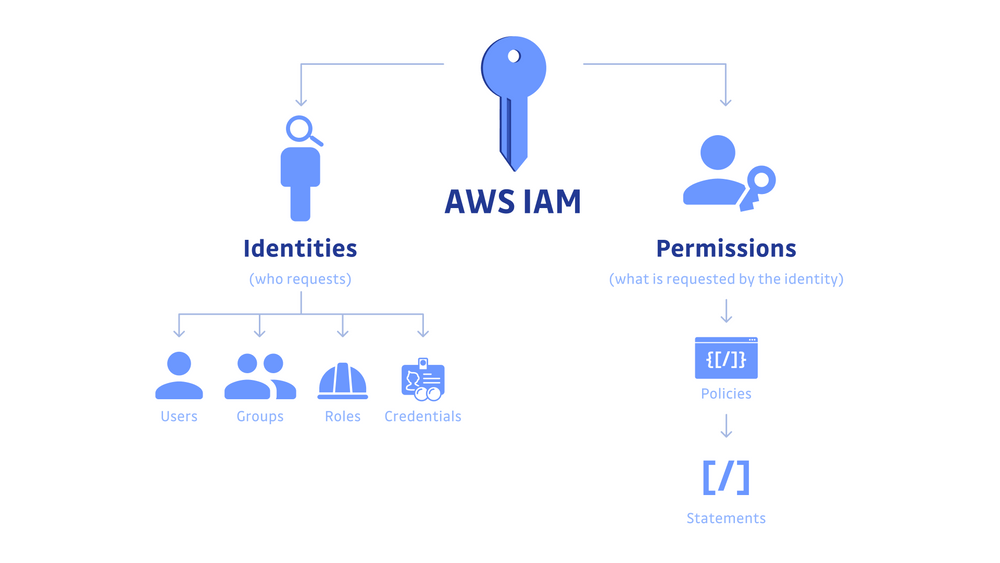
\includegraphics[width=\textwidth]{iaminfrastructure.png}
    \caption{Overview of AWS IAM concepts}{\cite{28}}
    \label{fig:iamidentities}
\end{figure}


\hfill \break

\textbf{Features of IAM}

\begin{itemize}
    \item \textbf{Granular permissions:} Based on the usage, permissions can be granted to different people to access
    different resources. For example, some users are granted complete access to Amazon DynamoDB ,Amazon S3, Amazon EC2, and other AWS services while other users are only
    provide permissions to administer some EC2 instances, read-only access to some S3 buckets but no other services \cite{27}.
\end{itemize}
\begin{itemize}
    \item \textbf{Multi-factor authentication (MFA):} To enable enhanced security of the AWS account, it is possible
    to enable
    two-factor authentication to the root account as well as to the individual users’ account. This ensures the AWS user along with providing the username and password for the account also provides a code from a configured device \cite{27}.
\end{itemize}
\begin{itemize}
    \item \textbf{Identity federation:} Identity federation is a system of trust between two parties used for the purpose of authenticating the users and sharing the information that is required for granting access to the resources.
    Users who have their password in the organization's
    corporate network or elsewhere such as in the
    internet identity provider are allowed to log in to the AWS console by the identity federation.
    For example, consider a scenario where there is a user who has logged into his google account and would like to use the AWS account, then identity federation helps AWS IAM to trust the authentication method.
    This authentication enables temporary access to the user’s AWS account \cite{27}.
\end{itemize}
\begin{itemize}
    \item \textbf{Password policy:} Password is used to authenticate a user’s account and a strict password policy
    can make it
    even more secure. IAM password policy allows for password rotation and resetting the password remotely. It is
    possible to set rules such as a password must contain a number, special characters, or special symbols \cite{27}.
\end{itemize}


\textbf{Amazon Elastic Compute Cloud (EC2)}

\par Amazon \gls{ec2} is one of the core services offered by
AWS
which
allows to rent virtual machine to run computer
applications. Amazon EC2 avoids upfront hardware setup investment, enabling faster development and deployment of applications. Amazon EC2 enables launching as few or as many virtual servers as needed, managing storage, and configuring security and networking. Amazon EC2 enables scaling uo or down based on the changes in the requirements or reduction in the need to forecast traffic, and spikes in popularity \cite{29}.

\par Amazon EC2 provides virtual server that are used for
running applications on the AWS infrastructure. This
virtual server is called an EC2 instance and they come in different configurations of storage, memory, CPU, and networking resources to suit user needs. EC2 instances can be used for any computing task, for example as a web server. An AWS user can create, launch, and terminate an instance based on the need, paying by the second for active servers and hence the term elastic. In order to provide high level of redundancy and optimize latency, Amazon EC2 provides users with control over the geographical location of instances. Placing all of the instances into the same AZ will likely give us the best latency between them. When an EC2 instance is provisioned, by default each instance is assigned automatically a DNS name and a public and private IPV4 address \cite{30}.


\textbf{Features of EC2}
\begin{itemize}
    \item \textbf{Elastic Web-Scale Computing:} Amazon EC2 enables users to expand the capacity as per their needs within minutes, not hours or days.
    Users can simultaneously commission one, hundreds, or even thousands of server instances.
    It is possible to run many servers in
    parallel
    with these instances.
    Amazon EC2, user can decrease or increase the
    automation as per their needs \cite{31}.
\end{itemize}

\begin{itemize}
    \item \textbf{Versatile cloud hosting services:} Amazon EC2 gives users the choice to select from a variety of software packages, os, and types of instances.
    Amazon EC2 allows selecting a configuration of memory, instance storage, CPU, and boot partition size that is optimal for your choice of operating system and application. For example, the operating system options include a variety of Linux variants as well as Microsoft Windows Server \cite{29}.
\end{itemize}

\begin{itemize}
    \item \textbf{Security:} Cloud security is the highest priority at AWS. Amazon works with the Amazon VPC to provide additional security, isolating resources, and robust networking for the compute resources.
    The compute instances in AWS are located in the VPC in the specific IP range.
    Further, the user decides which instances are exposed
    to the internet and which remain private \cite{31}.
\end{itemize}

\begin{itemize}
    \item \textbf{Conjunction with other Amazon web
    services:} Amazon EC2 collaborates with most AWS
    services such as Amazon RDS, Amazon VPC, Amazon SQS, and Amazon S3 to provide a complete, secure, comprehensive solution for
    computation, query processing, and cloud storage
    across a wide range of applications \cite{31}.
\end{itemize}

\begin{itemize}
    \item \textbf{Completely controlled:} Users have
    complete control over the instances including root
    access and the ability to interact with instances just like any other system. Users can stop the instance while keeping the data on the boot partition, and then restart it using web service APIs. Using web service APIs makes it possible to reboot the instances remotely \cite{31}.
\end{itemize}

\textbf{Amazon Machine Image (AMI)}

\par An Amazon Machine Image (AMI) is a maintained and
supported image provided by AWS. An AMI provides the necessary information required for launching an instance. An AMI must be specified while launching an instance. It is possible to launch multiple instances of the same configuration from a single AMI. When instances of different configurations need to be launched, different AMI must be used \cite{32}.

\begin{figure}
    \centering
    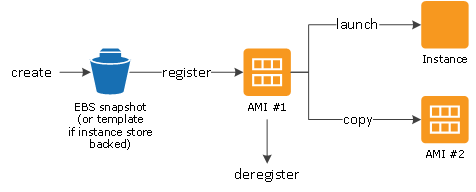
\includegraphics[width=\textwidth]{ami.png}
    \caption{Amazon Machine Image}{\cite{32}}
    \label{fig:ami}
\end{figure}

\par An AMI includes \cite{32}:
\begin{itemize}
    \item One or multiple Amazon \gls{ebs} snapshots or a
    template for the root volume of the instance, for instance-store-backed AMIs (for example, an application server, an operating system, and applications).
\end{itemize}
\begin{itemize}
    \item Launch permission in order to control which AWS accounts can use the AMI to launch instances.
\end{itemize}
\begin{itemize}
    \item A block device mapping that specifies to which instance the volumes must be attached when it’s launched.
\end{itemize}



\par Figure \ref{fig:ami} shows the lifecycle of AMI. The
Amazon Machine Image (AMI) is stored in an Amazon S3
bucket after it is created. This image is then registered and can then be used to launch a new instance. An AMI can be
copied to the same as well as to different AWS regions.
The AMI can be deregistered, if it is no longer required.
Upon deregistration a new instances cannot be launched
using the AMI, but the existing instances using AMI will
not be affected \cite{32}.

\par It is possible to launch an instance using an existing AMI. If the instance is customized, for example, the
software is installed on the image, this customized AMI can be saved with the updated configuration. Launching an
instance from this customized image contains customizations that were made earlier. To restrict the availability of
an AMI it can be made private, alternatively, the AMI is
made public when the access doesn’t need to be restricted \cite{33}.


\hfill \break

\textbf{Instance metadata and user data}
\par Instance metadata is the data associated with your EC2 instance.
The \gls{imds} used instance metadata to configure and
manage
the
running instance.
IMDS can be accessed by each EC2 instance.
The instance metadata is divided into different categories such as events, hostnames, and security
groups. Instance metadata service contains information
about the running EC2 instance and can be used to capture the temporary API credentials for accessing the AWS APIs \cite{34}.

\par Instance metadata can be used to access user data that is specified when launching the instance. For example, it
is possible to specify parameters for configuring the instance or include a simple script. It is also possible to
build generic AMIs and use user data to modify the configuration files supplied at launch time.
When more than one instance is launched at the same time,
the user data is available to all instances.
Each instance has a unique number called the ami-launch-index number.
This number allows for writing code that controls what to
do.
For example, the first host might elect itself as the original node in a cluster \cite{34}.


\hfill \break

\textbf{Amazon Relational Database Service (RDS)}

\par Amazon \gls{rds} is a set of managed services that
make it
easy
to
set up, operate, and scale databases in the Amazon Web Services Cloud.
An array of database engines to organize and store data
are supported by Amazon RDS.
An array of database engines is supported by Amazon RDS for organizing and storing the data.
Performing management tasks such as data patching, migration, recovery, and back up is also supported by Amazon RDS.
Amazon RDS provides its users access to the functionality of a familiar MariaDB, MySQL, SQL Server, Oracle, or PostgreSQL database.
Maintenance and deployment of relational databases in the cloud are facilitated by Amazon RDS.
Figure \ref{fig:rds} shows the different database
services offered by Amazon RDS. Amazon RDS manages common database administration tasks and provides cost-efficient, resizable capacity for an industry-standard relational database.
Based of various database use cases, Amazon RDS provides users an opportunity to choose an instance type that meets their needs.
The database instance varies with respect to the memory,
CPU, network capacity, and storage, thus providing
flexibility in choosing the ideal combination of resources for your database \cite{35}.
\begin{figure}
    \centering
    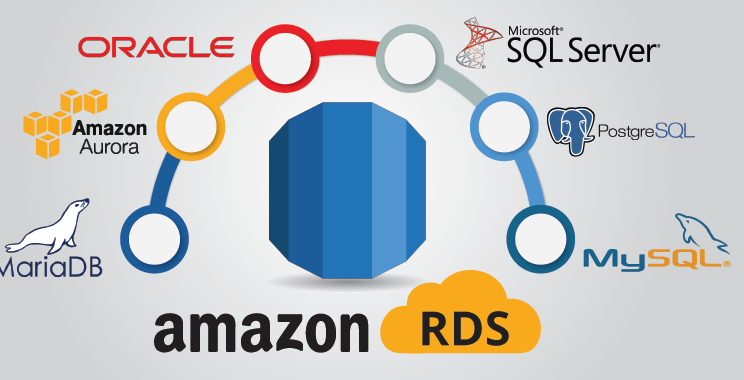
\includegraphics[width=\textwidth]{rds.png}
    \caption{Relational Database Service}{\cite{36}}
    \label{fig:rds}
\end{figure}

\par The pricing of Amazon Relational Database Service is based on usage.
The cost is dependent on various parameters such as instance hours, the number of input and output transactions, storage capacity, size of backup storage, or amount of Internet data transfer.
Different applications use different instance types.
The database instance is a fundamental element of the
Amazon RDS. A database engine works in each database instance with function parameters and specific properties that determine and control the properties of the databases. Database instances can be created, configured, and deleted using the AWS CLI, AWS management console, or RDS API. Computing and storage and capacity, database engine, and other parameters such as backup, version and update settings, or master user access data must be specified for each database instance. Depending on the type of database engine the number of databases per instance varies for example, with Microsoft SQL Server, up to 100 databases are possible, Oracle allows one database per instance, MySQL, MariaDB, Amazon Aurora, and PostgreSQL have no software limitations on the maximum number of databases \cite{37}.

\par Security of Amazon RDS and the stored or transmitted data is implemented at various levels.
AWS IAM controls which application or which user has access to which database resources and functions.
Depending on the requirements, groups and users are created and specific access rights are assigned.
Database instances are in a protected Amazon \gls{vpc}.
The access to the traffic that flows in and out of a DB instance is controlled by the VPC security groups.
The access to the DB instance is turned off by default.
In order to improvise security, access to the DB instance can be restricted to a specific IP address range, port or security group.
This can be achieved by specifying rules in a security group.
A total of 20 rules can be specified in a security group.
Once the rules are configured, every DB instance associated with that security group follows the same rules.
VPC security groups define which devices or instances can connect to a database instance.
The connections are encrypted and secured using Transport Layer Security (TLS) / Secure Sockets Layer (SSL) or IPsec VPNs. Amazon RDS firewall settings control network access. Database data at rest can be encrypted and database events can be logged \cite{71}.

\textbf{Features of RDS Instances}
\begin{itemize}
    \item \textbf{Amazon RDS Resources Encryption:} Data that is encrypted includes the underlying storage for DB instances, its automated backups, snapshots, and read replicas.
    The industry standard AES-256 encryption algorithm is used by the Amazon RDS encrypted DB instances to encrypt the data that is stored on the DB instances.
    After the data encryption is enabled, with minimal impact on the performance Amazon RDS handles decryption of data and authentication of access transparently.
    There is no modification needed in the database client to use encryption \cite{37}.
\end{itemize}
\begin{itemize}
    \item \textbf{Automatic backups:} Amazon RDS provisions creation and saving automatic backups of RDS DB instance.
    It
    provides users the capability choose a retention period and restore databases to any time during that period.
    Users can also take snapshots of instances manually and these snapshots remains until manually deleted \cite{37}.
\end{itemize}
\begin{itemize}
    \item \textbf{Replication:} Amazon RDS uses built-in
    replication functionality of Microsoft SQL Server, Oracle, MariaDB, and PostgreSQL DB engines to create a read replica, which is a special type of DB instance, from the source DB instance.
    A read replica represents a copy of the actual instance that reflects changes to the actual in almost real time and under normal circumstances.
    Figure \ref{fig:readreplicasworking} shows a pictorial view of the working of read replica \cite{37}.
\end{itemize}
\begin{figure}
    \centering
    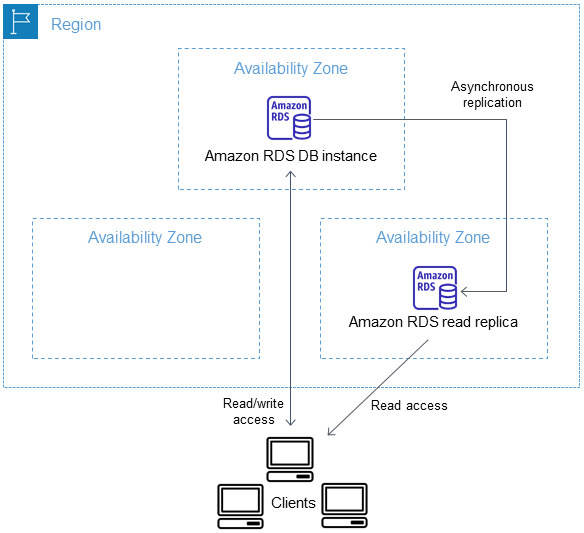
\includegraphics[width=\textwidth]{readreplicasworking.png}
    \caption{AWS RDS DB Instance Replication}{\cite{38}}
    \label{fig:readreplicasworking}
\end{figure}
\begin{itemize}
    \item \textbf{Performance metrics and monitoring:} Amazon provides CloudWatch service that enables managed
    monitoring.
    Amazon CloudWatch make it possible for the users to
    view capacity and I/O metrics \cite{37}.
\end{itemize}



\textbf{Amazon Simple Storage Service (S3)}

\par Amazon \gls{s3} is a high-speed, scalable, object
storage
service
in cloud that offers data availability, security and high performance.
Amazon S3 enables backup and archiving of data and
applications in AWS. It can store any type of object,
which allows uses like storage for Internet applications, data archives, backups, disaster recovery, hybrid cloud storage, IoT devices, and data lakes for analytics \cite{39}.

\par Storing, organizing, and retrieving data in Amazon S3 primarily focuses on two key components: objects and buckets that work together to create the storage system.
The Amazon S3 object storage data model is a flat structure.
The bucket stores the objects, once the bucket is created.
There is no real hierarchy of sub buckets or subfolders but a logical hierarchy can be inferred using key name prefixes and delimiters.
The objects are data files which include photos,
documents, and videos. Each object in the S3 environment
is identified by a unique key that differentiates it from other objects. The buckets serve as the fundamental storage containers for objects. While creating the bucket AWS provides users the ability to choose the AWS region. Even though a bucket is associated with a specified region, the name of the bucket acts as a global identifier, thus the name of the bucket must be unique among all the buckets across the world. The figure \ref{fig:s3} show Amazon S3, buckets and objects \cite{40}.

\par Amazon S3 offers features to organize and manage data to operate cost-effectively, support specific use cases,
increase security, and meet compliance requirements.
With S3 Versioning, it is possible to keep multiple variants of an object in the same bucket.
S3 Versioning helps to preserve, retrieve, and restore every version of every object stored in the buckets.
Amazon S3 generates a unique version ID once the S3 versioning in a bucket is enabled for each object added to the bucket.
Objects that already existed in the bucket at the time
versioning is enabled, such objects get assigned with a
version ID of \textit{null}. If an object is modified, such as \textit{CopyObject} and \textit{PutObject}, the new objects get a unique version ID \cite{41}.

\begin{figure}
    \centering
    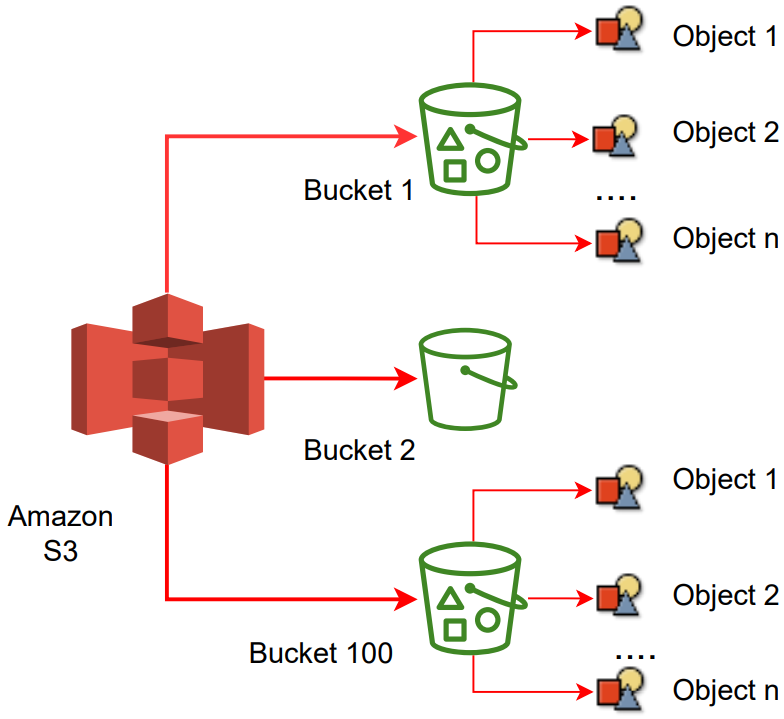
\includegraphics[width=\textwidth]{s3.png}
    \caption{Amazon Simple Storage Service}{\cite{42}}
    \label{fig:s3}
\end{figure}

\par Access to S3 objects is managed using the Identity
and access management service (IAM), bucket policies, S3
access points, and \gls{acl}.
With the Identity and access management service (IAM), it is possible to manage the access on the user or group level, it is also possible to delegate permissions to the S3 bucket to other AWS customer accounts.
To grant access permissions to the bucket and the objects, a resource-based AWS IAM policy called a bucket policy is used.
Associating a policy with a bucket can only be done by
the bucket owner.
JSON-based access policy language is used to create Bucket policies.
The bucket policies can be used to add or deny permissions for the objects in a bucket.
The way data can be accessed using that endpoint is
described by access points.
Amazon S3 Access Points describe how data can be accessed using that endpoint.
To perform S3 object operations such as
\textit{PutObject} and \textit{GetObject}, access points are
attached to buckets are used, .
Each S3 access point has its own access point policy.
To authorized users for individual objects and buckets, ACLs grants read and write permissions.
ACL are attached as a sub resource to each bucket and objects.
The ACL defines which AWS groups or accounts are granted access and the type of access to which the access is granted.
The Block Public Access feature in Amazon S3 provides settings for accounts, access points, and buckets to help user manage public access to resources.
By default, public access is not allowed on access
points, new buckets, and objects, however, users can
modify the access point policies, bucket policies, or object-related permissions to allow public access \cite{43}.

\par There are four settings provided by S3 Block Public
Access.
These settings can be applied in combination to individual buckets, access points, or entire AWS accounts. Upon applying a setting to an account, the setting is applied to all the access points and buckets that are owned by that account. Similarly, if the setting is applied to a bucket, it
applies to all access points associated with that bucket. Table \ref{tab:blockpublicaccesssettings} highlights
different settings for blocking public access \cite{23}.



\begin{longtable}{|p{5cm}|p{11.4cm}|}
    \hline
    \textbf{Name} & \textbf{Description} \\
    \hline
    \textit{BlockPublicAcls} & When BlockPublicAcls is set to TRUE the following behavior are seen:
    \begin{itemize}
        \item If the specified access control list (ACL) is public, PUT Bucket acl and PUT Object acl calls fail.
    \end{itemize}

    \begin{itemize}
        \item If the request includes a public ACL, PUT Object calls fail.
    \end{itemize}

    \begin{itemize}
        \item On applying this setting to the AWS account, then PUT bucket call fails in a situation where public ACL is included in the request.
    \end{itemize}
    \par When BlockPublicAcls is set to TRUE, the above specified operations fail, however, existing policies and ACLs for buckets and objects are not modified. This setting enables protecting against public access while allowing to audit, refine, or otherwise alter the existing policies and ACLs for buckets and objects \cite{44}.
    \\
    \hline
    \textit{IgnorePublicAcls} & Setting IgnorePublicAcls to TRUE causes Amazon S3 to ignore all public ACLs on a bucket and any objects it contains.
    This ensures the public access granted by ACLs will be blocked, while the PUT object calls that include a public ACL will still be allowed.
    The persistence of any existing ACLs does not get affected by enabling IgnorePublicAcls, and also it doesn't prevent new public ACLs from being set. \cite{44}.  \\
    \hline
    \textit{BlockPublicPolicy} & When BlockPublicPolicy is set to TRUE for a bucket, Amazon S3 rejects calls to PUT Bucket policy if the BlockPublicPolicy allows public access. When BlockPublicPolicy is set to TRUE for an access point, Amazon S3 rejects calls to PUT access point policy and PUT Bucket policy that are made through the access point if BlockPublicPolicy (for either the access point or the underlying bucket) is public \cite{44}.  \\
    \hline
    \textit{RestrictPublicBuckets} & The access to a bucket or access point with a public policy to authorized users and principals within the bucket owner's account will be restricted on setting RestrictPublicBuckets to TRUE.
    All cross account access to the bucket or access point are blocked by RestrictPublicBuckets, while it will still be possible for the users within the account to manage the bucket or access point \cite{44}.  \\
    \hline
    \caption{Block public access settings}
    \label{tab:blockpublicaccesssettings}
\end{longtable}

\textbf{Lambda:}
\par AWS Lambda is a serverless computing service that lets the users run code without provisioning or managing servers.
Lambda runs the code on a highly available compute
infrastructure and performs all the administrative tasks
of the compute resources, including capacity provisioning, code monitoring, server and operating system maintenance, automatic scaling, and logging \cite{45}.

\par With Lambda, it is possible to run code for virtually any type of application or backend service by supplying the code in one of the languages that Lambda supports.
The code is organized into Lambda functions.
From a few requests per day to hundreds or thousands of
request per second, lambda runs the function only when
needed and scales automatically.
Lambda functions are invoked using the Lambda API or as a response to an event from other AWS services.
There is no charge when the code is not running, users pay only for the compute time that Lambda consumes
When the code is not running, users don't get charged
and pays only for the compute time
that lambda consumes \cite{46}.

\par Lambda is an ideal compute service for many application scenarios, as long as the user can run the application code using the Lambda standard runtime environment and within the resources that Lambda provides.
When using Lambda, users are responsible only for their code.
Lambda manages the compute fleet of resources that offers a balance of memory, CPU, network, and other resources to run the code.
Because these resources are managed by Lambda, users cannot customize the operating system or login to compute instances on provided runtimes.
Lambda performs administrative and operational activities on behalf of users, including managing capacity, monitoring, and logging the Lambda functions.
AWS manages the entire infrastructure layer of AWS Lambda
and thus saves user time on operational tasks. AWS Lambda
provides a distinctive architectural property by enabling many instances of the same function, or of different functions from the same AWS account, to execute concurrently. This makes AWS Lambda a good fit for deploying highly scalable cloud computing solutions \cite{46}.

\par AWS Lambda invokes the function in an execution environment.
The execution environment provides an isolated and secure runtime environment and manages the resources required to run the function.
The support for any external extensions associated with the function or function's runtime is provided by execution environment.
The runtime of function and each external extension are
processes that run within the execution environment
\cite{46}.

\par The following phases are included in the execution
environment:
\begin{itemize}
    \item \textbf{Init phase}: In the init phase, Lambda unfreezes or creates an execution environment with the configured
    resources, downloads the code for the function and all layers, initializes the runtime, initializes any
    extensions, and then runs the function’s
    initialization code \cite{46}.
\end{itemize}
\begin{itemize}
    \item \textbf{Invoke phase}: During this phase, Lambda invokes the function handler. After the function runs to
    completion, Lambda prepares to handle another
    function invocation \cite{46}.
\end{itemize}
\begin{itemize}
    \item \textbf{Shutdown phase}: The shutdown phase is triggered if the Lambda function does not receive any invocations
    for a period of time.
    During the shutdown  phase, the runtime is shutdown
    by Lambda, it send an alert to each extension for
    stopping cleanly, and finally removed the environment \cite{46}.
\end{itemize}


\section{Security Framework}

\begin{figure}
    \centering
    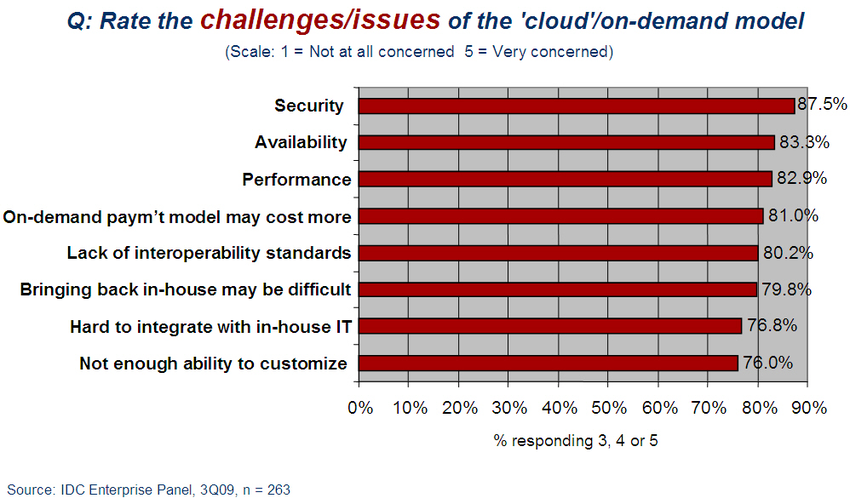
\includegraphics[width=\textwidth]{securitychallenges.png}
    \caption{Results of IDC ranking security
    challenges}{\cite{47}}
    \label{fig:securitychallenges}
\end{figure}

\par \gls{csp} leverage
virtualization technologies combined with self-service capabilities for computing resources via the Internet.
In these service provider environments, in order to maximize the efficiencies of virtualization, virtual machines must be located on the same physical server.
Based on a survey conducted by IDC as seen in the figure \ref{fig:securitychallenges}, of 263 IT executives and their line-of-business, security is ranked first as the greatest issue or challenge of cloud computing \cite{47}.

\par Information security management encompasses many areas from encryption and perimeter protection to application security and disaster recovery.
Security in IT is made more complex by compliance regulations, such as PCI, DSS, HIPAA, Sarbanes-Oxley, and global standards, such as GDPR. While most compliance experts and CEOs understand the value of cybersecurity measures, IT standards and security frameworks can make safeguarding organizations feel daunting.
Knowledge of standards, regulations, and frameworks is
essential for all infosec and cybersecurity professionals
\cite{48}.

\par A security framework is a compilation of international cybersecurity procedures and policies and state-mandated for maintaining and establishing security controls to protect critical infrastructure from cybersecurity risks.
These security frameworks are a blueprint for reducing vulnerabilities and managing risk by helping IT security professionals keep their organizations compliant and insulated from cyber threats.
The frameworks are used by Information security professionals to prioritize and define the tasks required to manage enterprise security.
It is possible for organizations to customize frameworks
to solve specific information security problems, such as
industry-specific requirements or different regulatory compliance goals \cite{48}.

\subsection{Prowler}

\par This research aims to introduce a framework called Prowler that can identify the security vulnerabilities or misconfigurations that exist in AWS accounts.
The thesis work focuses on the most popular AWS services,
IAM,
EC2, Lambda, S3, and RDS.
The introduced framework indicates to which security vulnerabilities the application is vulnerable and which security issues must be addressed to resolve the security vulnerability.
Prowler contains a set of controls, mapped against known security vulnerabilities, which can determine whether a given AWS cloud setup is vulnerable to these security vulnerabilities.
It aims to provide more in-depth security for AWS RDS,
EC2, IAM, S3, and Lambda resources and protects them
against security vulnerabilities.\\

\hfill \break
\par Prowler is an open-source AWS Security Best Practices Assessment, Hardening, Auditing, and Forensics Readiness command line tool.
Prowler scans the AWS account to check for potential security vulnerabilities, overly permissive Identity and Access Management (IAM) permissions, and best practice violations.
Using Prowler, it is possible to evaluate the AWS
security specifically against the CIS AWS Foundations
Benchmark and has more than 190 additional checks related
to \gls{hippa}, FFIEC, \gls{pci-dss}, SOC2, ISO-27001,
\gls{gdpr}
and
others \cite{49}.
Prowler provides more than 240 checks covering security best practices across all AWS regions and related to AWS services such as Amazon CloudFront, Amazon Redshift, Amazon ElasticCache, Amazon API Gateway, etc.
It helps organizations implement practices that ensure
having proper security measures in place and a secure
environment.
Prowler supports the generation of assessment reports in multiple formats such as JSON, CSV, HTML, JUnit, or JSON ASFF Security Hub.
The colorful or monochrome report enhances the user’s visibility.
Prowler also supports running a specific check or groups or creating your own.
When running the Prowler assessment, prowler supports
checking multiple AWS accounts in Parallel or
sequentially \cite{50}.\\
\hfill \break
\par Prowler is written in bash, and it uses AWS-CLI
underneath.
It works with multiple operating systems such
as macOS, Linux, or Windows with Cygwin or virtualization.
To use Prowler, though, an EC2 instance with the necessary security permissions can be provisioned, Fargate or any other container, CloudShell, Codebuild, and Cloud9.
Prowler can also be deployed directly in AWS using the AWS
CLI and other components such as Python pip,
detect-secrets, an open-source tool used to detect secrets by running scans, and jq , a flexible and lightweight command-line JSON processor already installed.
Detect-secrets is  \cite{50}.
\hfill \break
\begin{figure}
    \centering
    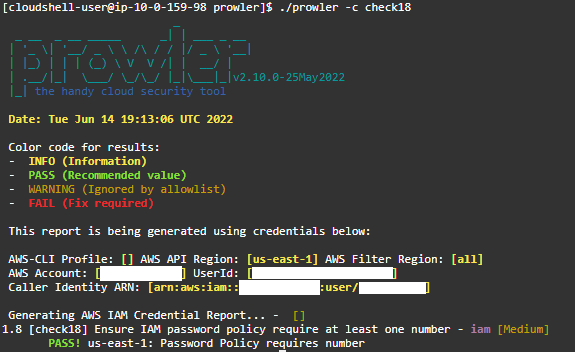
\includegraphics[width=\textwidth]{prowlercheckpass.png}
    \caption{Check execution in Prowler}
    \label{fig:prowlercheckexecution}
\end{figure}

\par After installing the required tools and packages
successfully, the AWS environment need be configured with
a valid Access Key and Region or by declaring the AWS
variables.
This can be done by running the command \textit{aws configure}.
In order to run all the Prowler checks, managed policies
\textit{SecurityAudit} and \textit{ViewOnlyAccess} must
be added to the user \cite{47}.



Prowler can then be installed directly by cloning the
code for the source repository \cite{48} using the
command \textit{git clone https://github.com/prowler-cloud/prowler} and does not require any additional setup afterward.
Once the source code is available, the assessment of security vulnerability using Prowler is performed by executing the command \textit{./prowler}.
Figure \ref{fig:prowlercheckexecution} shows the execution of the check using Prowler.
When the command is run, Prowler authenticates the configured environment variable.
Upon successful authentication, the checks are run over all the AWS regions.
To limit the assessment to a custom profile and region, the command \textit{./prowler -p custom-profile -r us-east-1} is used.
Prowler also enables assessing a single security vulnerability by running the command \textit{./prowler -c check78}.
The check78 is a check id, this check ensures there are no Public Accessible RDS instances (verifies publicly accessible RDS instances).
Table \ref{tab:prowlerextra} shows the execution result
of the assessment performed using Prowler \cite{48}.
\begin{table}[h!]
    \begin{center}
        \caption{Prowler check execution result}
        \label{tab:prowlerextra}
        \begin{tabular}{|p{1.4cm}|p{1.7cm}|p{1.5cm}|p{4.0cm}|p{5.0cm}|}
            \hline
            \textbf{Result} & \textbf{Severity} & \textbf{CheckID} & \textbf{Check Title} & \textbf{Check Output}\\
            \hline
            Pass & Critical & 7.8 & [extra78] Ensure there are no Public Accessible RDS instances &
            No Publicly Accessible RDS instances found\\
            \hline
        \end{tabular}
    \end{center}
\end{table}

\par If the user wants to save the assessment report for later analysis, Prowler enables saving the result in different formats such as CSV, JSON, Html, etc.
The command to generate the assessment report in CSV
format is
\textit{./prowler
-M csv} \cite{49}.

\begin{figure}
    \centering
    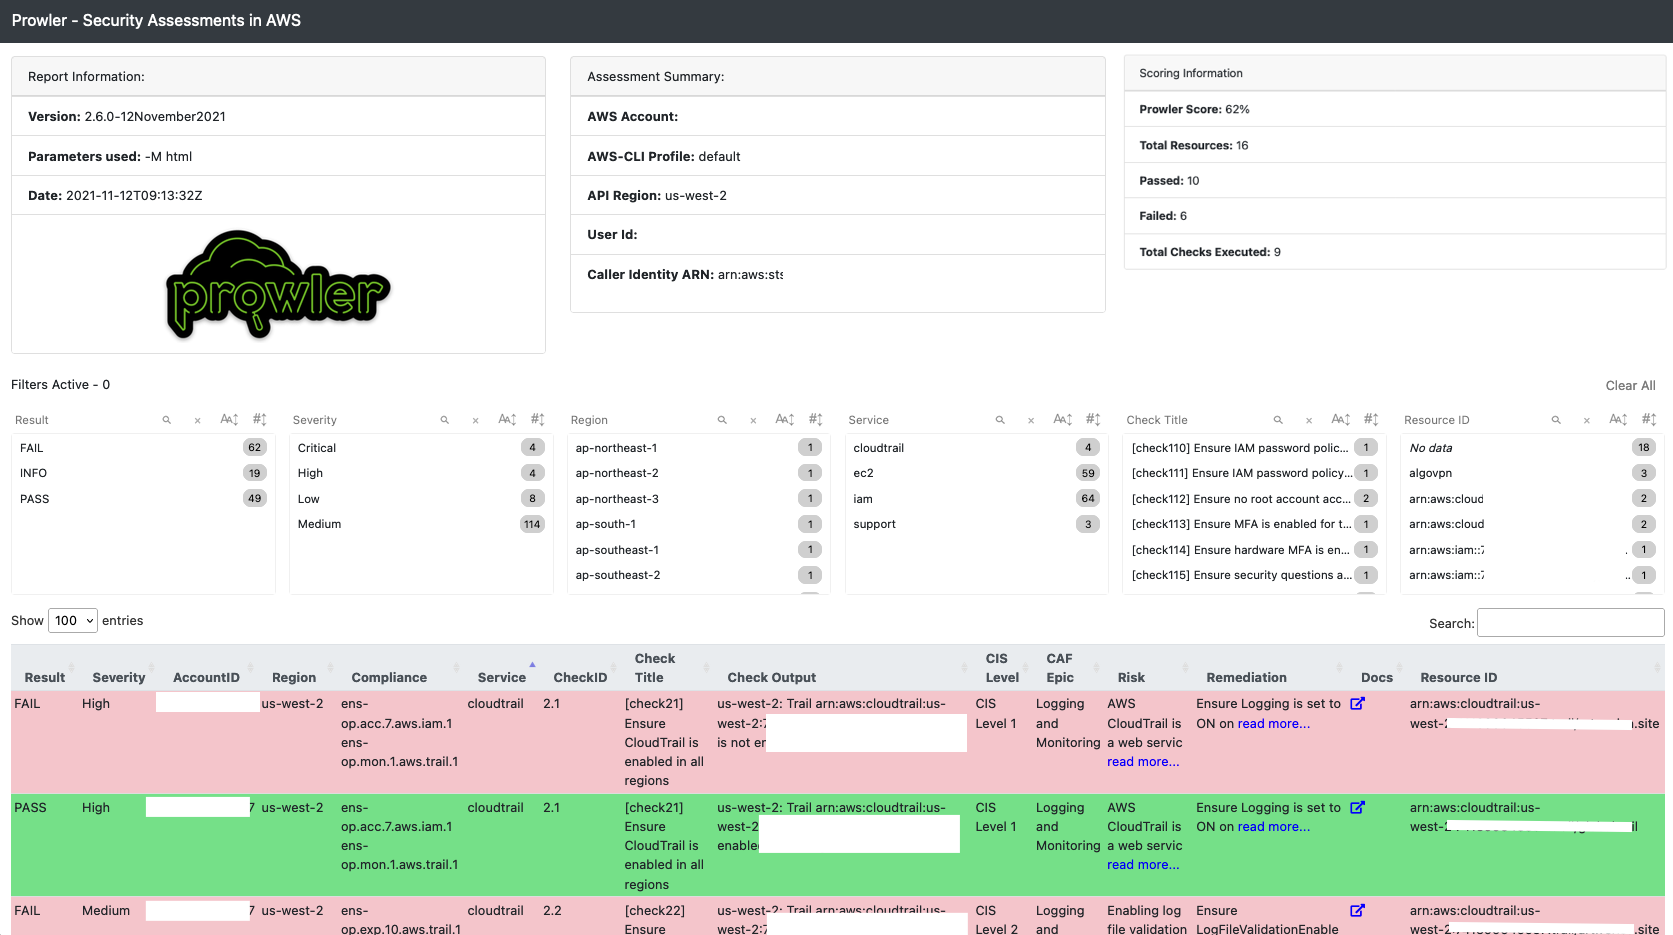
\includegraphics[width=\textwidth]{prowlerassessmentreport.png}
    \caption{Assessment report in Prowler}
    \label{fig:assessmentreport}
\end{figure}

The figure \ref{fig:assessmentreport} shows the
assessment report generated after the assessment of AWS
account using Prowler.